\chapter{Non-parametric analyses}
\label{nonParametric}
This chapter will not be considered until the next chapter on regression is complete, and this chapter is just a list of potential contents and the current contents are in pre-planning stages. I will also not review the details of every test (i.e. not go through the math, since I don't remember much of it), and will instead focus only on the basics: assumptions and pros/cons of the tests.

\section{Bootstrapping}
\label{bootstrap}

\subsection{Derek's problem}

In Section~\ref{poker}, Derek the poker player was introduced. His winnings are shown in Figure~\ref{pokerHistReprod}. His mean winnings of \$91 is positive, however, does this guarantee that he actually will make money in the long run if he plays professionally? A better question might be, does this estimate of the mean, \$91, precisely give his long term average?
\begin{figure}
\centering
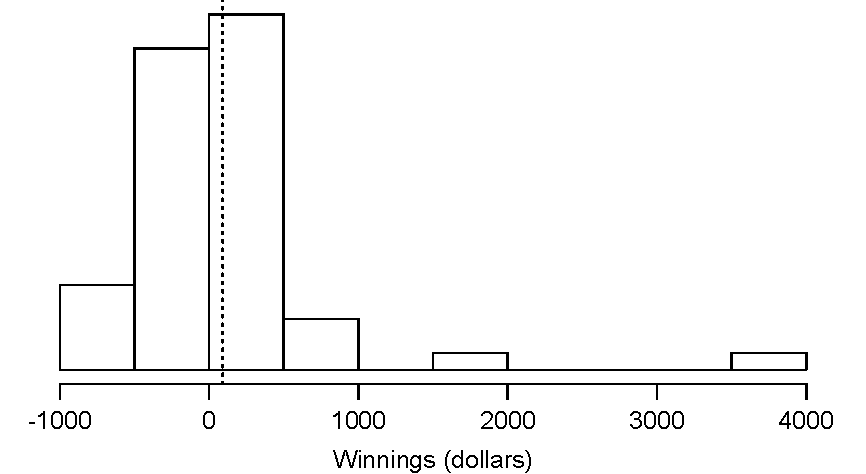
\includegraphics[height=1.9in]{ch6/pokerHistReprod/pokerHistReprod}
\caption{A histogram of Derek's poker winnings.}
\label{pokerHistReprod}
\end{figure}

In Section~\ref{basicsOfProbability}, Figure~\ref{dieProp} showed 100,000 simulations of rolling a die to get an estimate nearly indistinguishable from the probability $1/6$. How, with only 50 observations, can it be guaranteed that \$91 is the actual mean? Figure~\ref{pokerAverage} shows Derek's  average winnings over his 50 first days. Unlike the probability in Figure~\ref{dieProp}, the mean winnings do not settle down. Now how does \$91 sound as a highly accurate estimate of Derek's winnings?
\begin{figure}
\centering
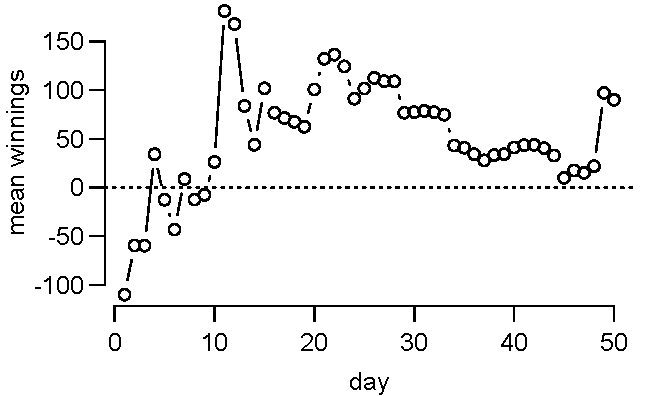
\includegraphics[height=1.9in]{ch6/pokerAverage/pokerAverage}
\caption{The running mean of Derek's poker winnings for his first 50 days.}
\label{pokerAverage}
\end{figure}

The difference in sample sizes in the probability example for Figure~\ref{dieProp} and Derek's winnings goes far to explain why one has ``settled'' and the other has not\footnote{There is still choppiness in the probability  data but it is not nearly as pronounced. In general, there will always be some choppiness in any sample's running average; that variability just gets smaller as the sample gets larger.}. If Derek would only take a (much) bigger sample, then there should be more settling.

So does Derek go back to the casino to gamble and collect more data? Not so fast. While there isn't an obvious way to say what Derek's long term average will be, this chapter is about starting to investigate this problem, without the need to get more data.

\subsection{Simulating $\bar{y}$}

While there is variability in $\bar{y}$, can it be somehow understood? Suppose that Derek's winnings could be simulated, then his 50 first days could be simulated many times and, of greater interest, the mean of the 50 first days could be simulated.

But the actual distribution isn't known, however, there is an estimate of this distribution: the sample itself.

One method is the bootstrap, which is a technique to simulate resampling. Instead of observed more new data, the already sampled data is recycled. To obtain a new simulated data set -- in this case of 50 days -- 50 observations are sampled from the already observed data \emph{with replacement}. Four such resampled distributions are shown in Figure~\ref{derekBootstrap4}. In each of these four samples, the simulated

\begin{figure}
\centering
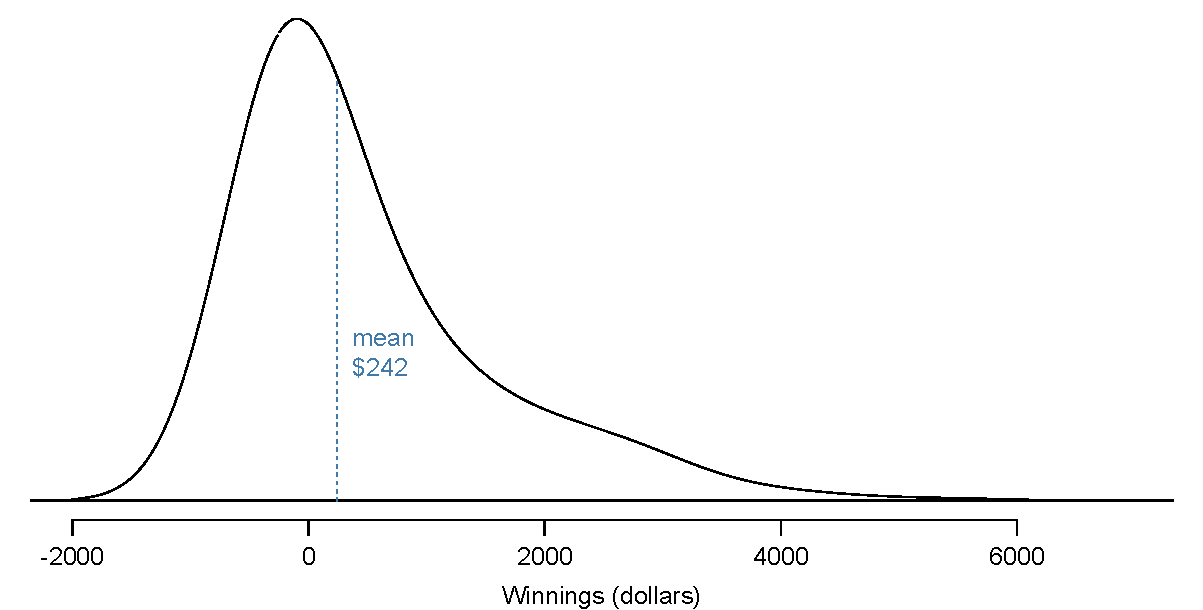
\includegraphics[height=1.9in]{ch6/pokerDistEst/pokerDistEst}
\caption{The running mean of Derek's poker winnings for his first 50 days.}
\label{pokerDistEst}
\end{figure}

\section{Randomization tests}
\subsection{Fisher's exact test}
\label{fisherTest}
\subsection{Wilcoxon signed-rank test}
\subsection{Two-sample Wilcoxon test}
\subsection{Paired Wilcoxon test}

\section{Kernel smoothing}

\section{Comparing distributions}
\subsection{Kolmogorov-Smirnov goodness of fit test}